\documentclass[10pt,final,journal]{IEEEtran}
\usepackage{xcolor} % Allows to make use and define many colors.
\usepackage[numbers]{natbib}
\usepackage{graphicx}
\usepackage{hyperref} 


%flowchart DOT code
%digraph G {
%	rankdir=LR
%	node [shape = rectangle]
	
%	a[label="Input video"]
%	b[label="Painting segmentation\n with bounding box"]
%	c[label="Painting transformation\n to standard format"]
%	d[label="Feature detection\n using brute force\n ORB matcher"]
%	e[label="Comparing feature vector\n against other paintings in dataset"]
%	f[label="Plot location of painting on ground plan"]
%	
%	a -> b [label="frames"]
%	b -> c [label="segmented painting"]
%	c -> d [label="painting in\n standard format"]
%	d -> e [label="feature vector"]
%	e -> f [label="match result"]
%	
%	{rank=same; a d}
%	{rank=same; b e}
%	{rank=same; c f}
%}


\newcommand{\todo}[1]{\color{red}\_ToDo: #1 \color{black}}
\graphicspath{{./img/}}
\title{Continuous room localisation using painting detection}
\author{Bert De Saffel, Timothy Thiecke}
\begin{document}
	\maketitle
	\begin{abstract}
		
		This paper describes our method to localise a painting on a ground plan based on The Musem of Fine Arts in Ghent. 
	\end{abstract}


	\section{Introduction}
	This paper introduces a framework for rapid painting detection.
	\todo{What makes this work useful?}
	
	\todo{Why should someone spend time to read this paper}
	
	\todo{clarification of title and context}
	
	\todo{which problem has been solved}
	
	\todo{overview of related work}
	
	\todo{benefits and shortcomings of related work}
	
	\todo{overview of your own contributions}
	This paper contains $x$ contributions:
	\todo{overview of results}
	
	\todo{why these results are useful}
	
	\todo{overview of structure of the paper}
	In section 2 ...

	
	Based on a frame from a camera which contains a painting, 
	
	Figure \ref{fig:groundplan_msk} shows the ground plan that is used to mark the correct room
	
	\begin{figure}
		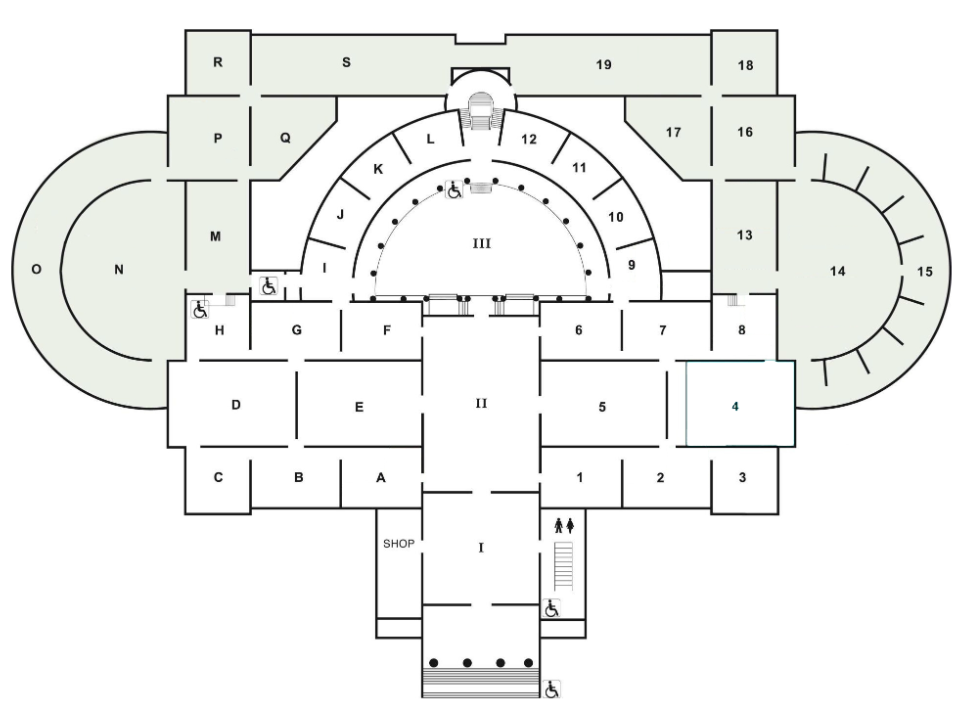
\includegraphics[width=\linewidth]{groundplan_msk}
		\caption{A ground plan of The Museum of Fine Arts, Ghent. }
		\label{fig:groundplan_msk}
	\end{figure}

	\section{Painting Detection}
	\todo{ook dingen uitleggen die niet werkte}
	\begin{itemize}
		\item \todo{vanishing points}
		\item \todo{hough transformatie}
		\item \todo{lijn intersectie}
		\item \todo{gabor filter}
		\item \todo{local binary patterns}
	\end{itemize}

	\todo{gebruik ook afbeeldingen}
	
	\subsection{Painting Segmentation}
	The first step of the algorithm is the segmentation of a painting in an arbitrary video frame. A typical painting contains the art on its own enclosed by a painting frame. This painting frame causes a strong change in environment, increasing the effectiveness of an edge detector. Extracting the edges with the Canny edge detector yields a first indication of where a painting might be. If the full painting frame is visible on the video frame, its contour can be calculated using \cite{SUZUKI198532} which returns a vector of points for each contour. We consider only contours which have four points.
	
	It is possible that multiple paintings exist on a single frame, 
	
	\subsection{Feature Detection}
	
	
	\subsection{Path Tracking}
	Once a painting is identified and matched, it can be localised on the ground plan. To achieve this, the ground plan is converted into a directed graph. The nodes of this graph are the rooms of the museum and the edges define the connections between rooms. When a user starts recording paintings, the matching algorithm will be performed on each frame and a location will be found. The graph is able to mark nodes in three distinct ways. A green node is the start of the path, an orange node is an intermediate path and the blue node is the end of the path. The path ends when the user stops recording. The path direction is also visualised by coloring the corresponding edges green. Note that when a cyclic path occurs which was walked in both directions, information of order is lost.
	
	
	
	
	To illustrate the path tracking algorithm,  a small segment consisting of rooms 1, 2, 3, 4, 5, 6, 7 and 8 are converted into such a graph and is show on figure \ref{fig:groundplan_msk_simple_graph}.
	
	
	%digraph G {
	%	2[fontcolor=white, fillcolor=green, style=filled]	
	%	4[fillcolor=orange, style=filled]
	%	5[fillcolor=orange, style=filled]
	%	7[fillcolor=orange, style=filled]
	%	6[fontcolor=white,fillcolor=blue, style=filled]
	%	1 -> 2
	%	2 -> 1
	%	2 -> 3
	%	2 -> 4[color=green]
	%	2 -> 5
	%	3 -> 2
	%	4 -> 2
	%	4 -> 5[color=green]
	%	4 -> 7
	%	4 -> 8
	%	5 -> 7[color=green]
	%	7 -> 6[color=green]
	%	6 -> 7
	%	7 -> 8
	%	7 -> 5
	%	7 -> 4
	%}

	\begin{figure}
		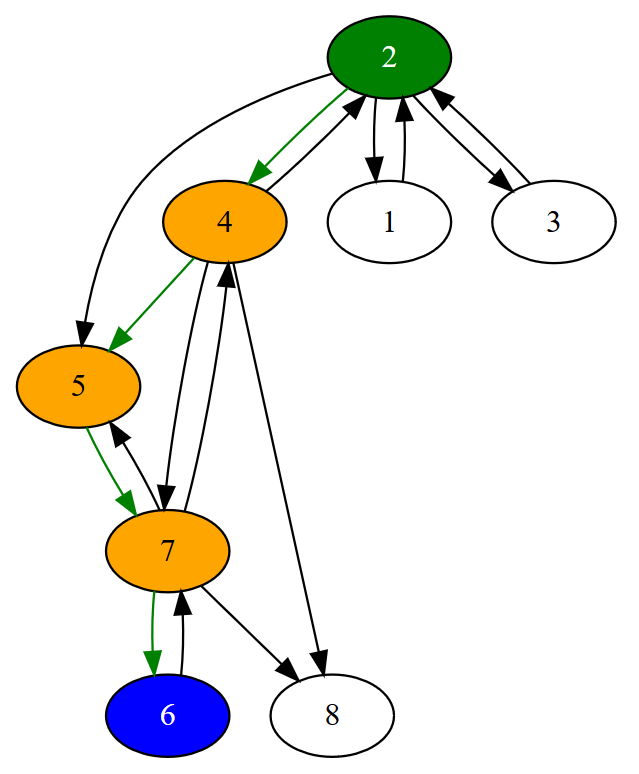
\includegraphics[width=\linewidth]{groundplan_msk_simple_graph}
		\caption{Path tracking using a graph. }
		\label{fig:groundplan_msk_simple_graph}
	\end{figure}
	
	\subsection{Database}
	The database consists of 688 images of various paintings and sculptures in the museum. In this work we only focus on the paintings of this dataset. The paintings were extracted from two different camera's: a Nokia 7 plus and a Samsung A3. Each image also contains the room in which it resides as metadata.  
	
	To reduce the load time of this database, a prebuilding stage was implemented. This stage reduces each image to a collection of interest points and corresponding descriptors for these interest points as generated by the ORB \cite{Rublee2011} algorithm. 
	
	
	\section{Evaluation}
	To measure the performance metrics of our algorithm, we employ three different methods: for painting segmentation, the matching algorithm and room localisation consistency. First, an evaulation of painting segmentation is done using a random sample of the dataset. In this sample, each painting is segmentated manually, resulting in four coördinates for each image. These coördinates can be compared against the coördinates that are generated by the painting segmentation algorithm. A distance metric is used to compare the closeness of two coördinates.
	
	The matching algorithm has to be evaluated manually by comparing the matcher's result. The correctness of the matching algorithm is simply the ratio of the correct matches against the false matches.
	
	To evaluate the room localisation, a sample of the video dataset was taken. The generated path is compared against the actaul path.
	
	
	
	
	
	
	\section{Results}
	\todo{qualitative as well as quantitative}
	
	\todo{quantitative: graphs, tables, roc-curves, f1-scores, ...}
	
	\todo{qualititative: technisch, show where and why the method succeeds or fails, pictures of easy and difficulty cases}
	
	\section{Conclusion}
	\todo{overview of the most important contributions and the results, without introducing anything new}
	
	\todo{after the reader has read the paper, the reader can look at the contributions and results from a different viewpoint}
	
	\todo{statements can be made more explicit}
	
	\todo{eventueel future work}

	\bibliographystyle{IEEEtran}
	\bibliography{IEEEabrv,library}
\end{document}